\documentclass{article}
\usepackage{amsmath,amsthm}
\usepackage{graphicx}
\usepackage{wrapfig}
\usepackage{url}
\usepackage{caption}
\usepackage{subcaption}
\usepackage[justification=centering]{caption}

\title{The dynamics of factored state hidden Markov models}
\date{1 December 2020}



\begin{document}

\maketitle

\begin{abstract}
The purpose of this expository note is to outline the possible use cases for factored hidden Markov models (fHMM) and to explore the current state-of-the art methods for inference and learning problems with fHMM.  We will discuss the cost and complexity of fHMM versus classical hidden Markov models and make the case for fHMMs as a critical tool for industrial data analysis.  
\end{abstract}

\section{Introduction}
An important task in machine learning is to detect the latent signals present in data that cannot necessarily be captured by the naked eye or by basic statistical methods.  When the data in question is sequential, then we have to consider not only the geometry of the data itself, but also the added dimension of time.  One tool that has proven quite successful in classifying latent states in sequential data has been the hidden Markov model (HMM), which takes advantage of the underlying Markov dynamics of the data; that is, we expect that the conditional probability distribution at the current timestep depends only on the timestep immediately preceeding it. If the data is generated by a single Markov process, then there are classical algorithms like the Baum-Welch expectation-maximization (EM) algorithm, or the Viterbi algorithm for the problems of learning and inference \cite{G01}.  However, as the data becomes more complicated, the problem of classification quickly becomes intractible using classical methods.

\subsection{A motivating example}

\begin{figure}
\centering
\begin{subfigure}{.5\textwidth}
  \centering
  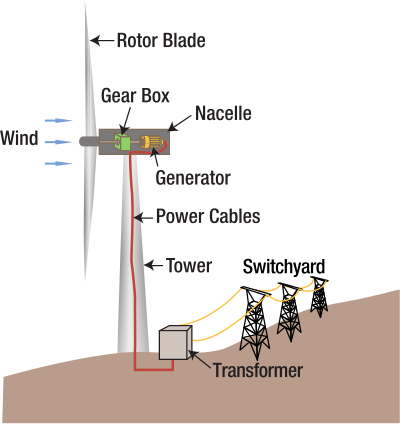
\includegraphics[width=.75\linewidth]{figures/full_turbine_parts.png}
  \caption{}
  \label{fig:full_turbine_parts}
\end{subfigure}%
\begin{subfigure}{.7\textwidth}
  \centering
  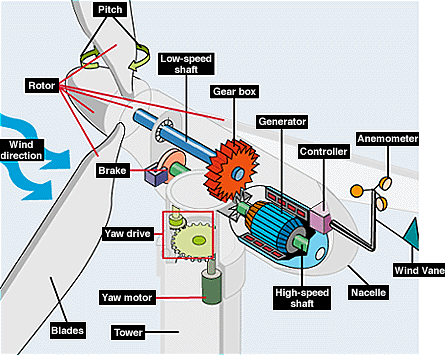
\includegraphics[width=.75\linewidth]{figures/turbine_parts.png}
  \caption{}
  \label{fig:turbine_parts}
\end{subfigure}
\caption{Labeled parts of (a) the wind turbine including the transformer and power cables \cite{U13} and (b) the wind turbine head \cite{MX12}.}
\label{fig:test}
\end{figure}

Let's consider the example of a windfarm with a fleet of 30 turbines, and let's suppose we want to model the operating status of a single wind turbine. The operating status can take on one of four values, 
\begin{align*}
h_1&=\text{``In Use - Normal"}\\
h_2&=\text{``In Use - Faulty"}\\ 
h_3&=\text{``In Maintenance Mode"}\\
h_4&=\text{``Not in Use".}  
\end{align*}
Suppose we have observations corresponding to features such as power generated, windspeed, rotational fequency, transformer temperature, and a categorical alarm value.  In principle the sequence of observations is evolving from a single underlying Markov process related to the status of the turbine, and this is borne out in each of the features.  In other words, we would expect each of the four hidden states to loosely correspond with a particular constellation of observations. If the underlying model dynamics are already known, then for a sequence of observations with length $T$, the most likely sequence of hidden states could be inferred with time complexity $O(TN^2)$ (where $N$, the number of latent states, is four in this case) using the Viterbi algorithm \cite{V67}, or even faster if various sampling methods are employed.  In that case where we don't already have meaningful model parameters, they can be learned relatively easily using the Baum-Welch EM algorithm.  The algorithm learns the optimal model parameters by iteratively applying an expectation step which involves a foward-backward computation of posterior probabilities over hidden states, and a maximization step which uses the posterior probabilties to maximize the complete data likelihood.  Effective implementations of both steps of the Baum-Welch algorithm exist; the expectation step has a time complexity equivalent to the Viterbi algorithm, and straighforward methods exists for effective execution of the maximization step.                    

Where the classical HMM suffers, is when the underlying dynamics of the data are governed by multiple processes that are perhaps losely coupled or where the evolution of features is occurring on much different scales.  For such an example suppose we wanted to more directly monitor the status of particular components of the wind turbine.  So, for example suppose we want to monitor the power cables, brake, yaw motor, generator, and transformer where each of these can have the status ``normal" or ``faulty".  If we were to proceed with a vanilla HMM as above we would be dealing with 32 hidden states.  In the best case scenario, if we were able to extract meaningful HMM parameters, inferring the proper sequence of hidden states would suffer under the quadratic time complexity of the Viterbi algorithm.  


In the more likely case, we would not even be able to extract meaningful HMM parameters from this scenario, since the dynamics governing the operating status of the brakes and the transformer, for example, are not tightly coupled.  Rather, they evolve independently, but with some conditional dependence.  Faulty brakes might increase the likelihood of downstream faults in the system, though the may arise for totally different reasons. Because of the complexity of this data, it is better modeled through a system of multiple conditonally dependent HMMs which we call a factored hidden Markov model (fHMM).  The fHMM in question will consist of five HMM layers, each with only two hidden states, which will decrease the complexity significantly as compared to a single 32 state HMM.

An fHMM is able to ``automatically decompose the state space into features that decouple the dynamics of the process that generated the data," \cite{GJ95} that is, we can hope to learn the Markov dynamics of the five different systems while using the complexity of the data to our advantage.  Once the fHMM parameters are known, we can then infer the most likely operational status for each of the five components using sampling methods or variational inference. 

In the following section we will introduce the preliminary definitions and notation necessary to describe the fHMM.  Then, we will discuss some problems related to the effectiveness of various alternative algorithms for learning and inference with fHMM.

\subsection{Preliminary notation and definitions}

\begin{figure}[t]
\centering
\begin{subfigure}{0.75\textwidth}
   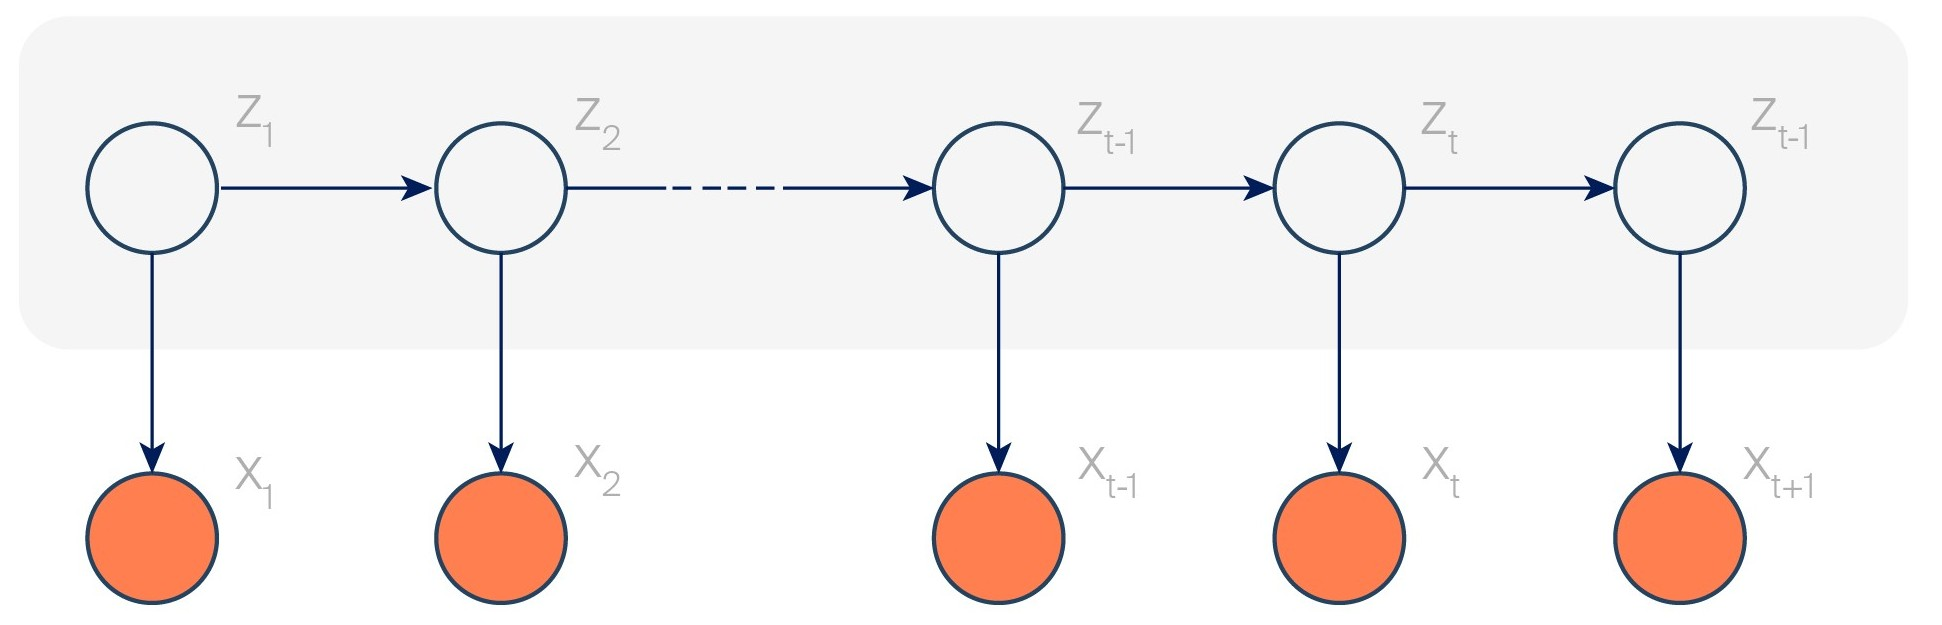
\includegraphics[width=1\linewidth]{figures/hmm.jpg}
   \caption{}
   \label{fig:hmm} 
\end{subfigure}

\begin{subfigure}{1\textwidth}
   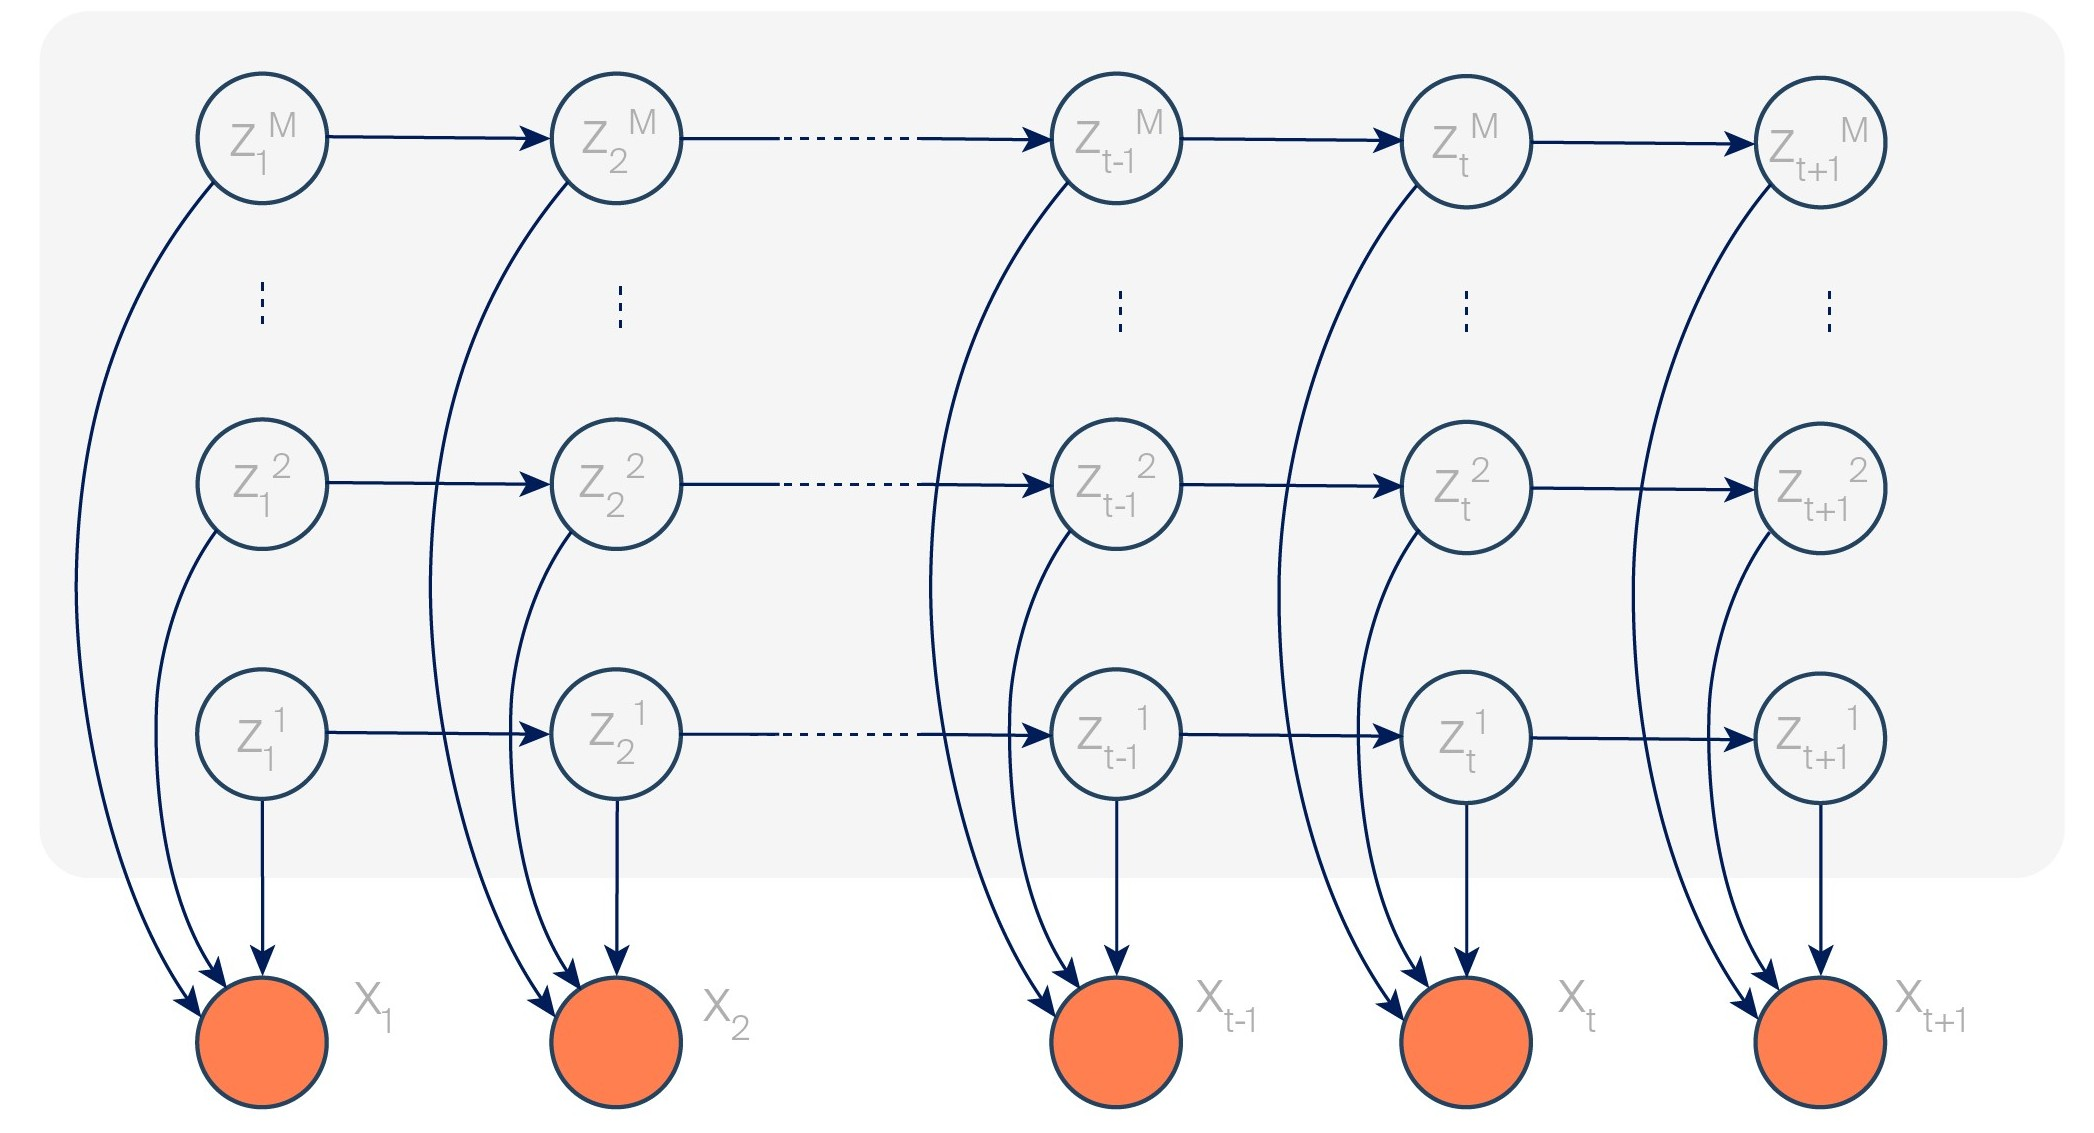
\includegraphics[width=1\linewidth]{figures/fhmm.jpg}
   \caption{}
   \label{fig:fhmm}
\end{subfigure}

\caption[Two numerical solutions]{Graphical representations of the classical hidden Markov model (a) and factored hidden Markov model (b).}
\end{figure}

Suppose we have a sequence of observations, 
\[
X = X_1,...,X_T
\]
where at each time $t$, the observation is a $k$ dimensional vector
\[
X_T = (x_{t,1},...,x_{t,K}),
\] 
whose entries can be drawn from continuous or discrete distributions, or a combination of the two.  
A hidden Markov model (HMM) is a latent state model that captures the Markov dynamics of a latent process underlying the observed data.  In its most basic form, the HMM models a sequence of hidden states
\[
Z = Z_1,...,Z_T
\]
corresponding to $X$, where for any time $t$, we have $Z_t\in \mathcal H$, with 
\[
\mathcal{H} = \{h_1,...,h_N\},
\]
although it's possible to draw hidden states from more complicated probability distributions (see, for example, Chapter 13 of Bishop's canonical text on the topic \cite{B06}).  The classical HMM can be described by three basic parameters.  The first is its initial state probability, which is a $N\times 1$ vector describing the probabilty of inhabiting each of the $N$ hidden states at time $t=1$.  The second is the transition probability that describes the likelihood of transitioning from any one state to another.  The transition probability is captured in an $N\times N$ matrix, 
\[
A = \begin{bmatrix}
a_{ij}
\end{bmatrix}_{1\leq i,j\leq N}
\]
where $a_{ij}$ is the probability of transitioning from hidden states $i$ to hidden state $j$ from one timestep to the next.  The third is its emission probability, which directly couples the observation sequence and the hidden state sequence and captures the probability of an observation vector given each of the hidden states. If the data is categorical them the emission probability can be expressed in terms of a matrix and in the case where the data is continuous then the emission probability needs to capture the full parameters of the probability distribution.

If the data in $X$ is generated by a single underlying process whose dynamics evolve on a uniform scale, then we expect the HMM to perform very well at the tasks of learning these model parameters and predicting the most likey sequence of hidden states. 

In an fHMM with $M$ underlying Markov processes, the hidden state, $Z_t$, at time $t$, is an $M$-dimensional vector,
\[
(z_{t}^{(1)},...,z_{t}^{(M)}) \in \mathcal{H}^{(1)}\times ...\times \mathcal{H}^{(M)}
\]
where 
\[
\mathcal H_m = \{h_1^{(m)},...,h_{N_M}^{(m)}\}, 
\]
is the space of discrete hidden states for all $1\leq m\leq M$.  To simplify the exposition, we will assume throughout this note that 
\[
N = N_1 = ...= N_M.
\]
A comprehensive treatment of fHMMs can be found in the foundational publication on the topic by Gharamani and Jordan \cite{GJ95}, but we will highlight some key components of that paper here.  The transition probability will now be captured in a collection of $M$ many $N\times N$ matrices, where
\[
A^{(m)} = \begin{bmatrix}
a_{ij}^{(m)}
\end{bmatrix}_{1\leq i,j\leq N}
\]
for $1\leq m\leq M$, where $a_{ij}^{(m)}$ is the probability of transitioning from hidden states $i$ of system $m$ to hidden state $j$ of system $m$ from one timestep to the next.  The probability of transitioning from one hidden state vector to another can then be constructed as a tensor product of these matrices.  More concretely, the probabilty of transitioning from a particular hidden state vector at time $t$ to any another hidden state vector at time $t+1$ can be decomposed as the product
\begin{eqnarray}\label{transition}
P\left((z_{t+1}^{(1)},...,z_{t+1}^{(M)}) \mid (z_{t}^{(1)},...,z_{t}^{(M)})\right) = \prod_{m=1}^M P(z_{t+1}^{(m)} \mid z_{t}^{(m)}).
\end{eqnarray}
In this way each of the Markov processes evolves independently, according to its own dynamics. 

Although we want to maintain this marginal independence for the hidden states, $Z$, we would expect some dependence once we condition on the observation sequence, $X$.  To understand the intuition behind this, let's revisit our example of involving the five components of the wind turbine.  While we don't expect the status of the generator from time $t$ to $t+1$ to be connected to the status of the yaw motor from time $t$ to $t+1$,if we were to observe a power surge that causes the generator to experience a fault, that might increase the likelihood that the yaw motor experiences a fault.  If we consider the fHMM as a graphical model as in figure (\ref{fig:fhmm}) we can couch this observation in the language of directed graphs and the so-called d-separation criterion. Without describing any of the technical details, we will simply point out that this conditional dependence means that we would not expect the emission probability to decompose as a tensor product as in (\ref{transition}).

\section{Model learning and inference for fHMM}\label{problems}
In the following sections we outline three concrete problems related to learning and inference with fHMM and provide some context of the current progress towards solutions to these probelms.
\subsection{Classical HMM methods}

The fHMM described in the previous section can always be flattened into an HMM with $M^N$ many hidden states, taking the transition matrix to be the full $M^N\times M^N$ matrix of transition probabilties.  For small $M$ and $N$ this might be a resonable choice, since the training and inference methods for classical HMMs are so straightforward (for a full derivation of these methods see \cite{HVB20}).  However, we can see from Table 1 of \cite{GJ95} that this method of flattening leads to model overfitting and overall poor performance which gets increasingly worse as $M$ and $N$ grow. Moreover, Figure 4 of \cite{GJ95} we see that even for $M=5$ and $N=3$ the time per iteration of EM becomes impractically slow.  To demonstrate this phenomenon, we propose the following analysis: 

\begin{quote}
\textbf{Problem 1:} Generate a sequence of synthetic data, $X$, with underlying fHMM structure.\footnote{A flexible implementation of a generative fHMM model already exists in the Tagup codebase}  Sampling model parameters from a uniform $[0,1]$ distribution, and normalizing so that the additive constraints are satisfied, and also varying over numbers of hidden states, we will determine the best possible complete data likelihood for a classical HMM trained on $X$. 
\end{quote}
Problem 1 will demonstrate that HMM training for complicated data will be very slow, it will yield a very low likelihood, or both.  The goal of this analysis will be to show that handling data which is generated by multiple underlying processes using a classical HMM will lead to very poor model performance, therefore making the case for more complicated methods of training and inference.  

\subsection{Bayesian inference and sampling methods}

In cases where exact inference is intractible, sampling methods that rely the principles of Bayesian inference can often be a reasonable approach for model training and inference.  The broad class of Markov chain Monte Carlo (MCMC) sampling methods includes many sampling algorithms that are effective in the case of classical HMMs. The general strategy of MCMC sampling methods is to draw samples from the space of model parameters at random and decide based on an acceptance criterion whether a sample will be retained and added to the posterior probability.  Gathering statistics along the way, such sampling methods can lead to effective model training, and in practice converge relatively quickly.  The precise formulation of the random walk and the acceptance criterion lead to various different algorithms of this type.  The Python package PyMC3 \cite{SWF16} comes equipped with a range of probability distributions and includes implementations of Gibbs \cite{CG92}, No U-Turn \cite{HG14} and Hamiltonian Monte Carlo \cite{DKPR87} samplers.  This leads to the following practical problems:

\begin{quote}
\textbf{Problem 2:} Using a combination of off-the-shelf and hand-coded sampling tools, use the principles of Bayesian inference to learn the model parameters of first an HMM and then an fHMM.\footnote{My understanding is that such implementations already exist for various configurations of classical HMMs, but I'm not sure of the extent to which these methods have been implemented for factored fHMMs.}  Use these implementations to solve inference probelms of the sequence of synthetic data, $X$, which we know to have underlying fHMM dynamics.
\end{quote}  
With the solution of problems 1 and 2 we will be able to demonstrate the effectiveness of Bayesian inference and sampling methods to solve training and inference probelms that were previous intractible, and demonstate the ability to capture the complex underlying dynamics that we know to be present in the data.

\subsection{Variational Inference}
In cases where $M$, $N$ or the underlying dataset are large, even the sampling methods described above can fail to fully capture the dynamics of the fHMM and become impractically slow.  In these cases, we turn to the tools of variational inference. For this class of inference, rather than iteratively improving our log likelihood by directly computing the posterior, we approximate the posterior distribution with an easy to understand distribution, and use this apprpximation to bound the log likelihood from below. For classical HMMs, learning and inference using stochastic variational inference with variable elimination algorithm is implemented in Numpyro \cite{B18,U19}.  Recently, so-called black box variational inference (BBVI) \cite{DA15} has become the state-of-the-art for stochastic variational inference since it uses Autograd to perform fast autodifferentiation to overcome some of the practical hurdles of variational inference.  Various implementations of various components of BBVI for HMM and fHMM exist but not in any way that's immediately useable for modeling large complex datasets.  Therefore, we have the following concrete goal:

\begin{quote}
\textbf{Problem 3:} Write an implementation of BBVI for fHMM learning and inference and demonstrate the utlitity of this implementation on the sequence of synthetic data, $X$, which we know to have underlying fHMM dynamics.
\end{quote}  
An implementation of BBVI for fHMM should allow for a fast data analysis that is impossible with exact inference methods or Bayesian inference based sampling methods.

\section{Conclusion}

The goal of Problems 1 outlined in Section \ref{problems} above is to demonstrate the limitations  of inference using classical HMM methods to analyze data which is generated by multiple losely-coupled Markov processes.  With the resolution of problems 2 and 3 we hope to develop working implementations of inference tools that are able to more effectively analyise this type of data.    

\bibliographystyle{siam}
\bibliography{references}

\end{document}

A factored HMM with 
